\begin{figure}[ht] % [especificador de posições]:exemplos [htbp] - h:aqui, t:topo, b:baixo, p:página especial, !: desconsiderar parâmetros internos
\begin{center}
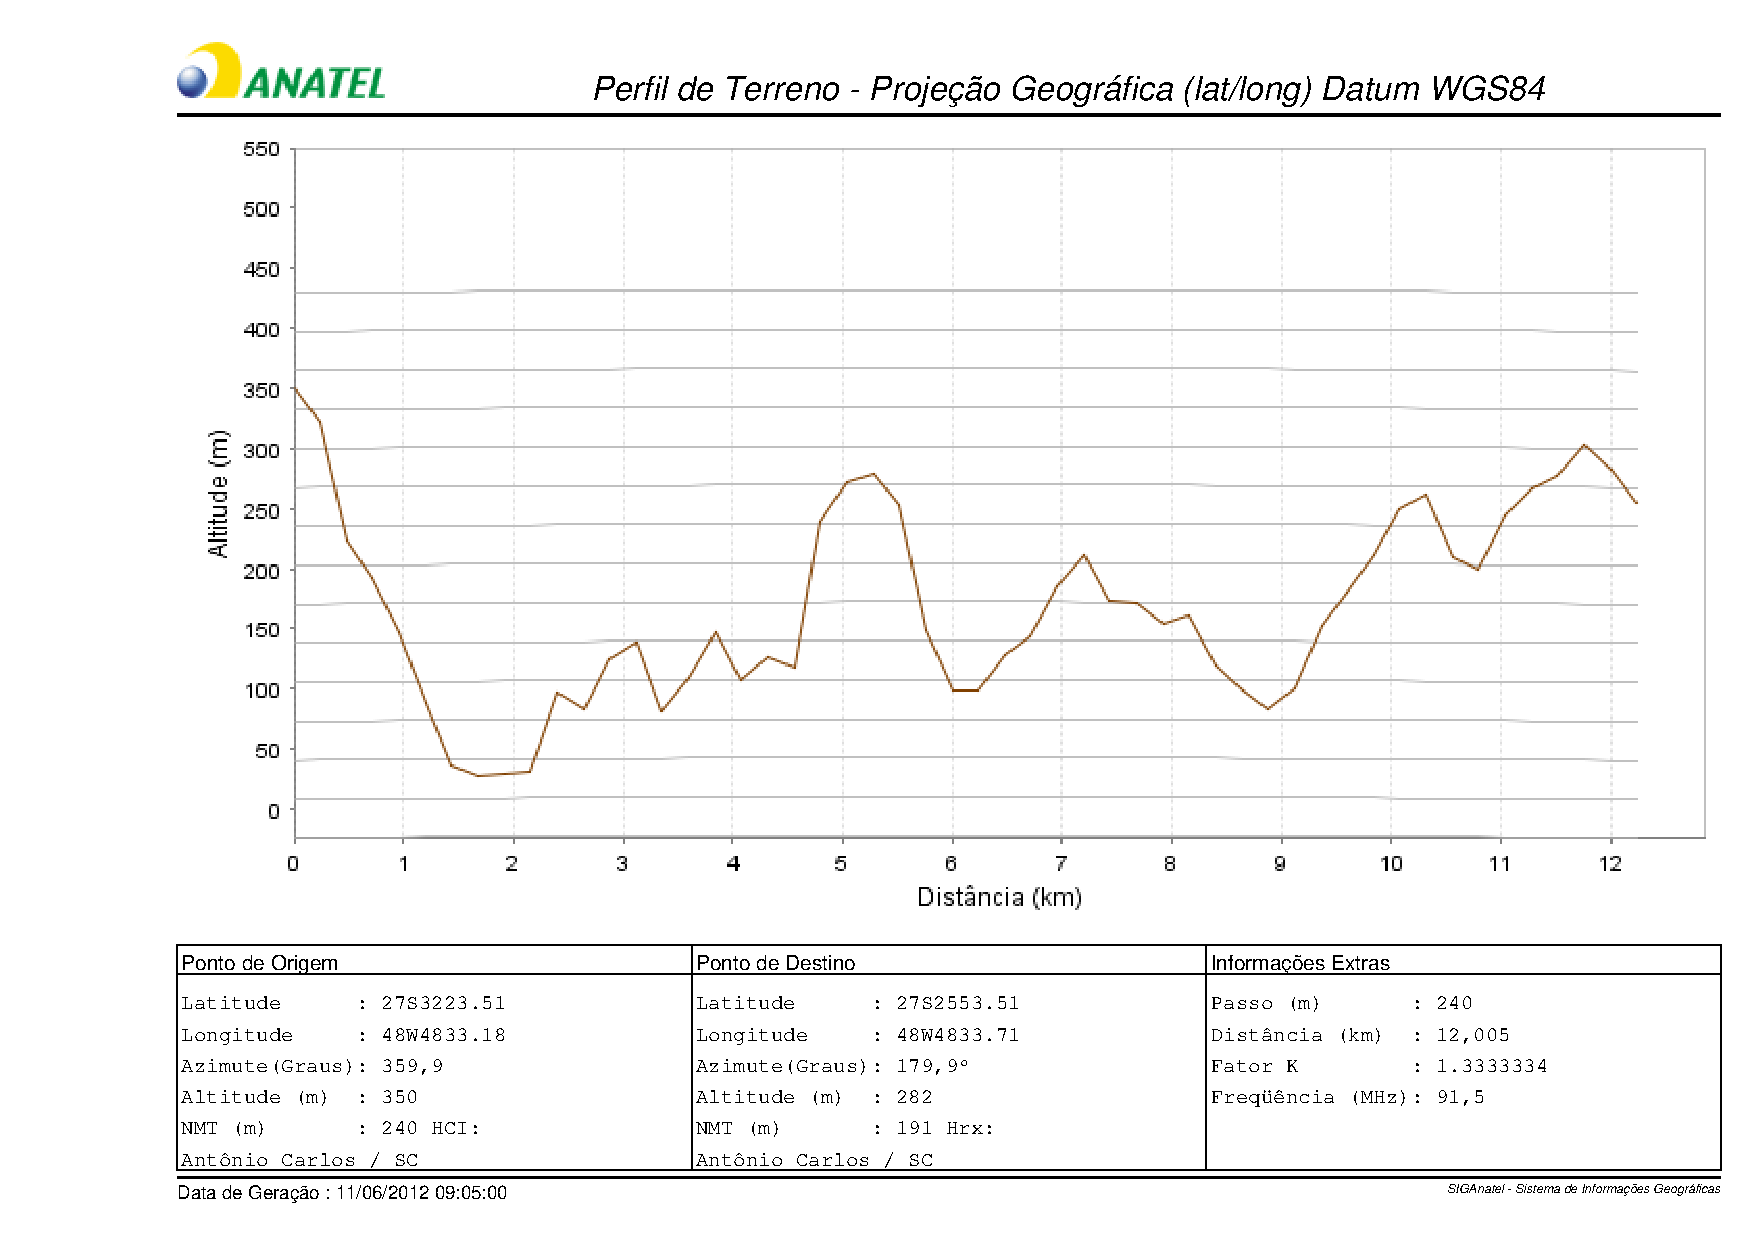
\includegraphics[scale=.5]{./figuras/nmt1_v2.pdf} %Opções width (largura em pt ou cm ou vezes se não houver unidade de medida), height (altura em pt, cm ou vezes se não houver unidade de medida), angle (rotação em graus), scale (escala em vezes 0.5= 50%,1.5=150%, etc )

%\caption{Radial 1}
Radial 1

\end{center}
\label{nmt1}
\end{figure}

\begin{figure}[ht] % [especificador de posições]:exemplos [htbp] - h:aqui, t:topo, b:baixo, p:página especial, !: desconsiderar parâmetros internos
\begin{center}
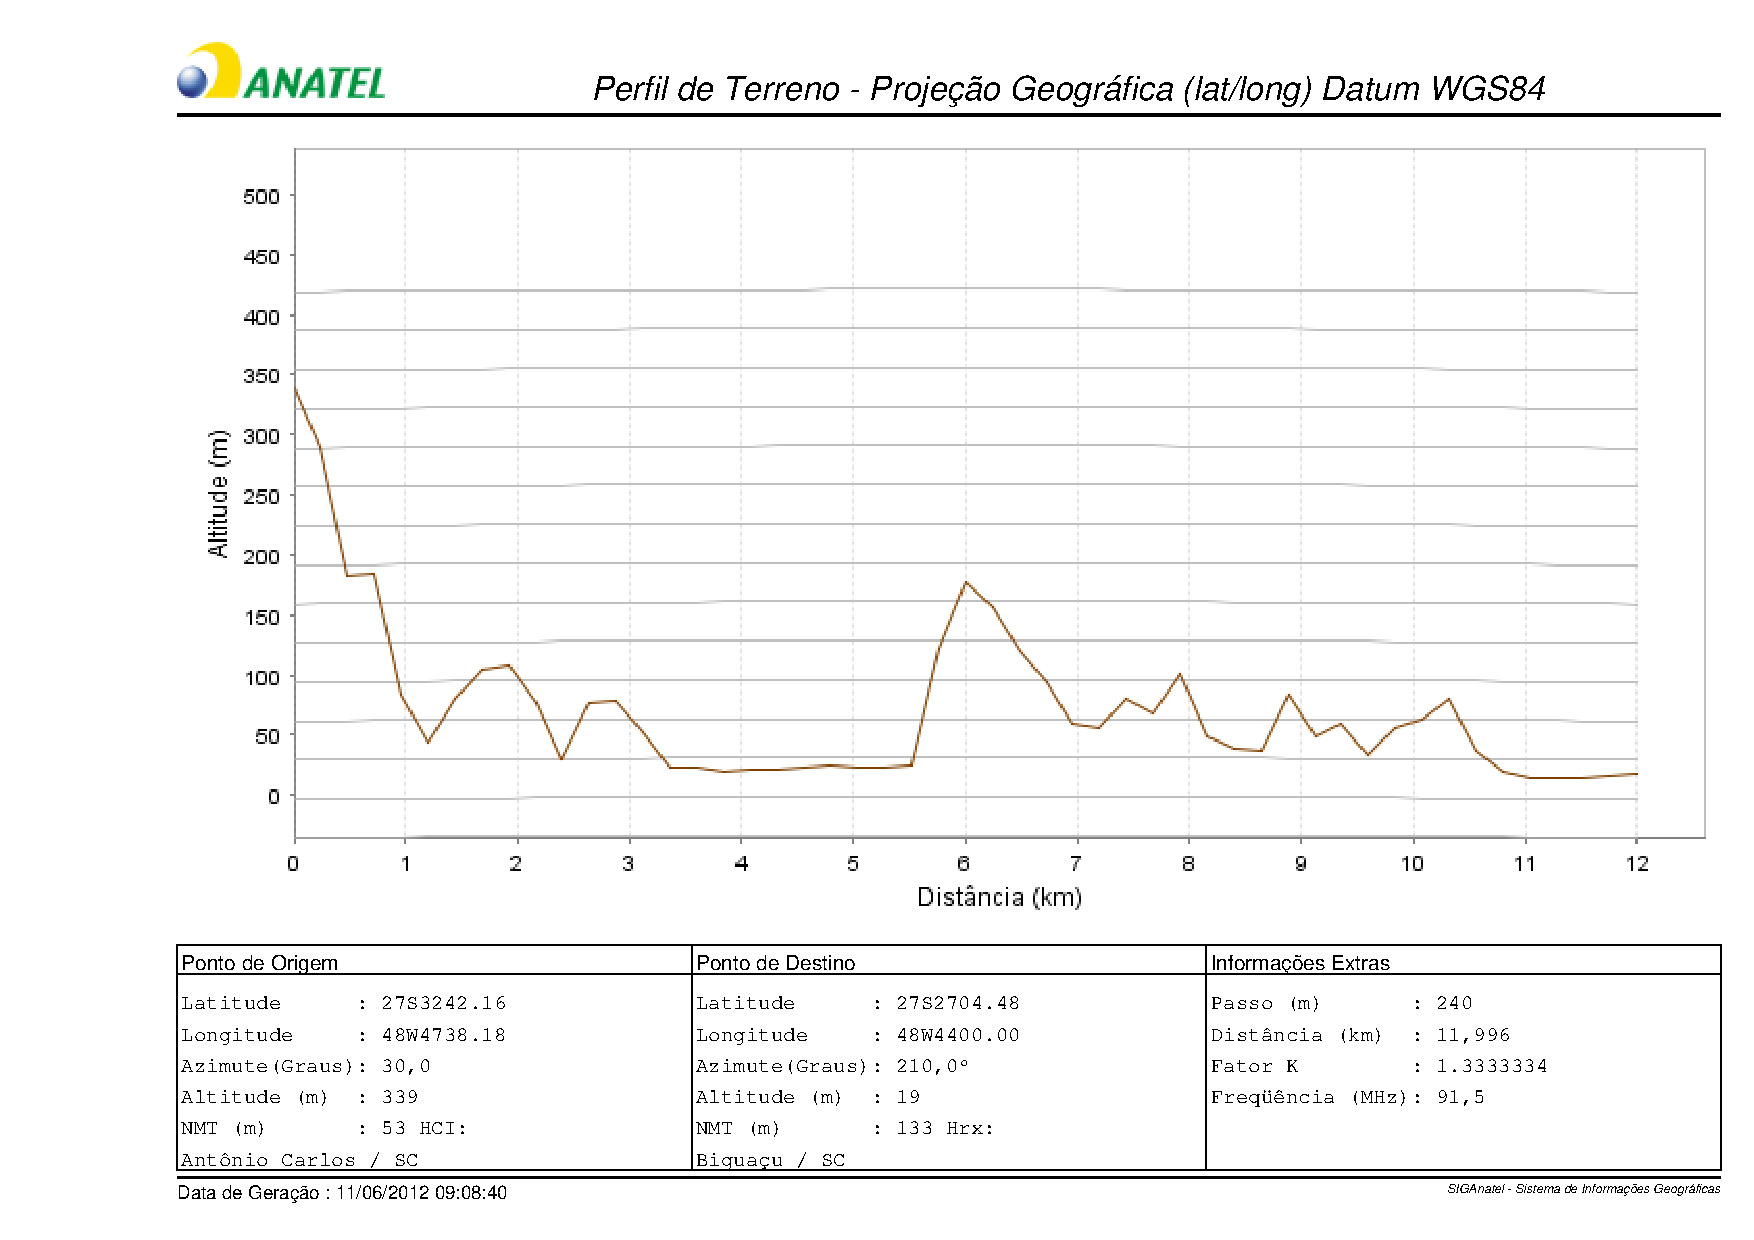
\includegraphics[scale=.5]{./figuras/nmt2_v2.pdf} %Opções width (largura em pt ou cm ou vezes se não houver unidade de medida), height (altura em pt, cm ou vezes se não houver unidade de medida), angle (rotação em graus), scale (escala em vezes 0.5= 50%,1.5=150%, etc )

%\caption{Radial 2}
Radial 2
\end{center}
\label{nmt2}
\end{figure}

\begin{figure}[ht] % [especificador de posições]:exemplos [htbp] - h:aqui, t:topo, b:baixo, p:página especial, !: desconsiderar parâmetros internos
\begin{center}
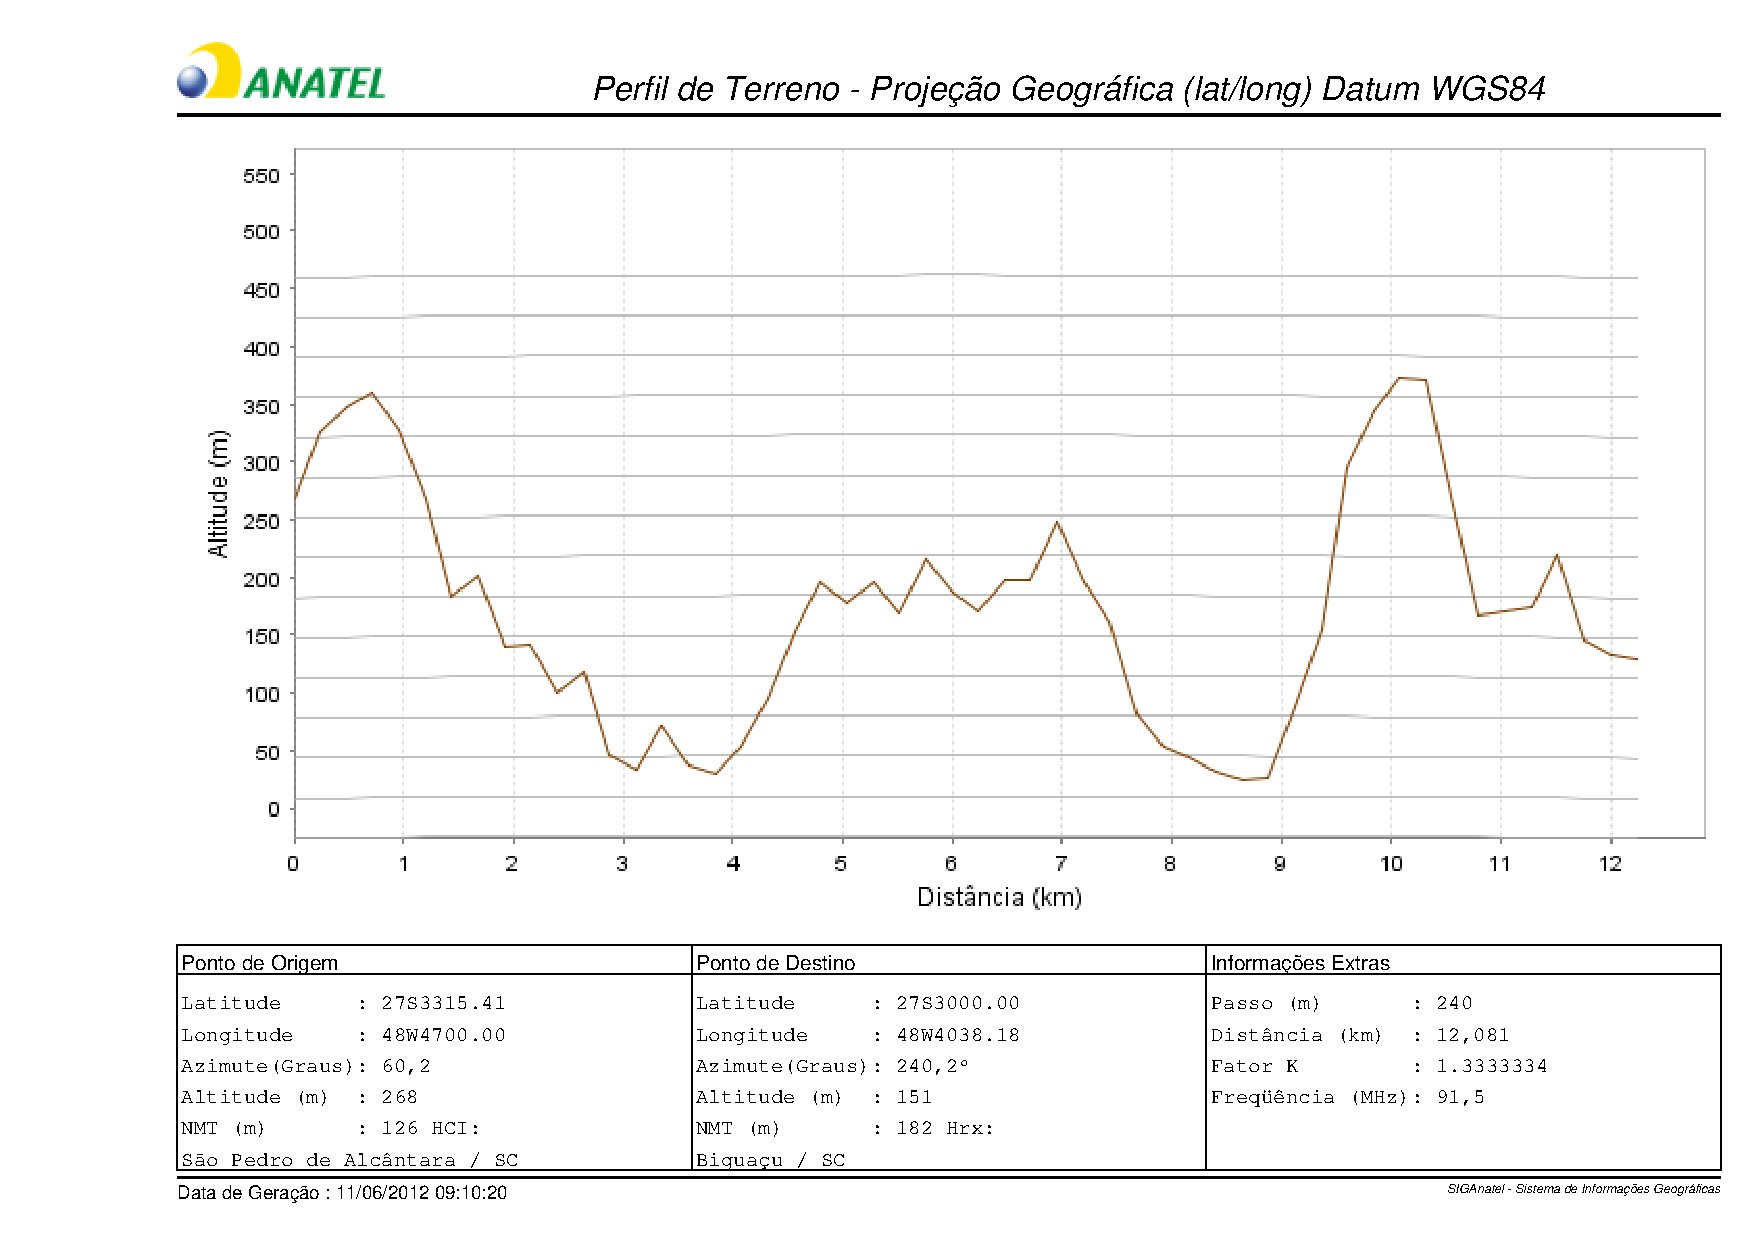
\includegraphics[scale=.5]{./figuras/nmt3_v2.pdf} %Opções width (largura em pt ou cm ou vezes se não houver unidade de medida), height (altura em pt, cm ou vezes se não houver unidade de medida), angle (rotação em graus), scale (escala em vezes 0.5= 50%,1.5=150%, etc )

%\caption{Radial 3}
Radial 3
\end{center}
\label{nmt3}
\end{figure}

\begin{figure}[ht] % [especificador de posições]:exemplos [htbp] - h:aqui, t:topo, b:baixo, p:página especial, !: desconsiderar parâmetros internos
\begin{center}
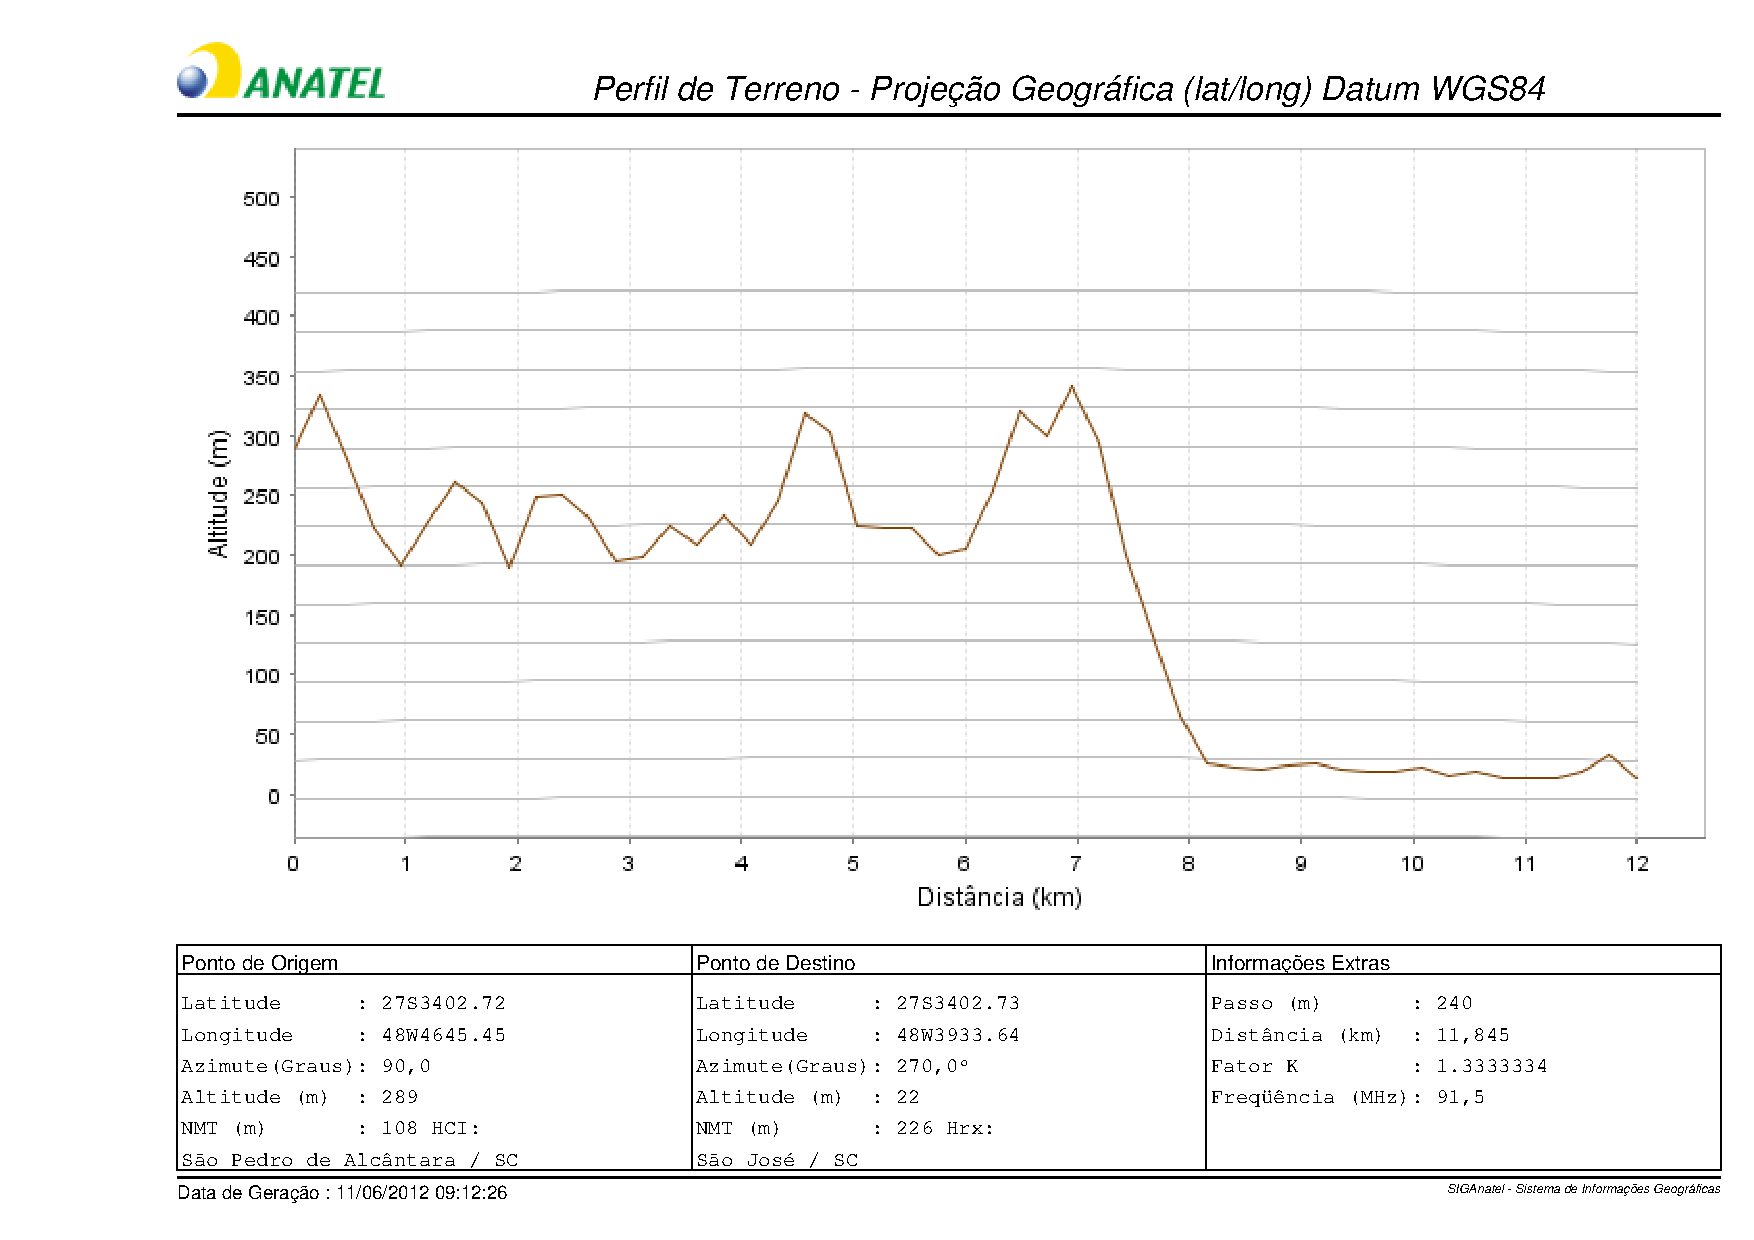
\includegraphics[scale=.5]{./figuras/nmt4_v2.pdf} %Opções width (largura em pt ou cm ou vezes se não houver unidade de medida), height (altura em pt, cm ou vezes se não houver unidade de medida), angle (rotação em graus), scale (escala em vezes 0.5= 50%,1.5=150%, etc )

%\caption{Radial 4}
Radial 4
\end{center}
\label{nmt4}
\end{figure}

\begin{figure}[ht] % [especificador de posições]:exemplos [htbp] - h:aqui, t:topo, b:baixo, p:página especial, !: desconsiderar parâmetros internos
\begin{center}
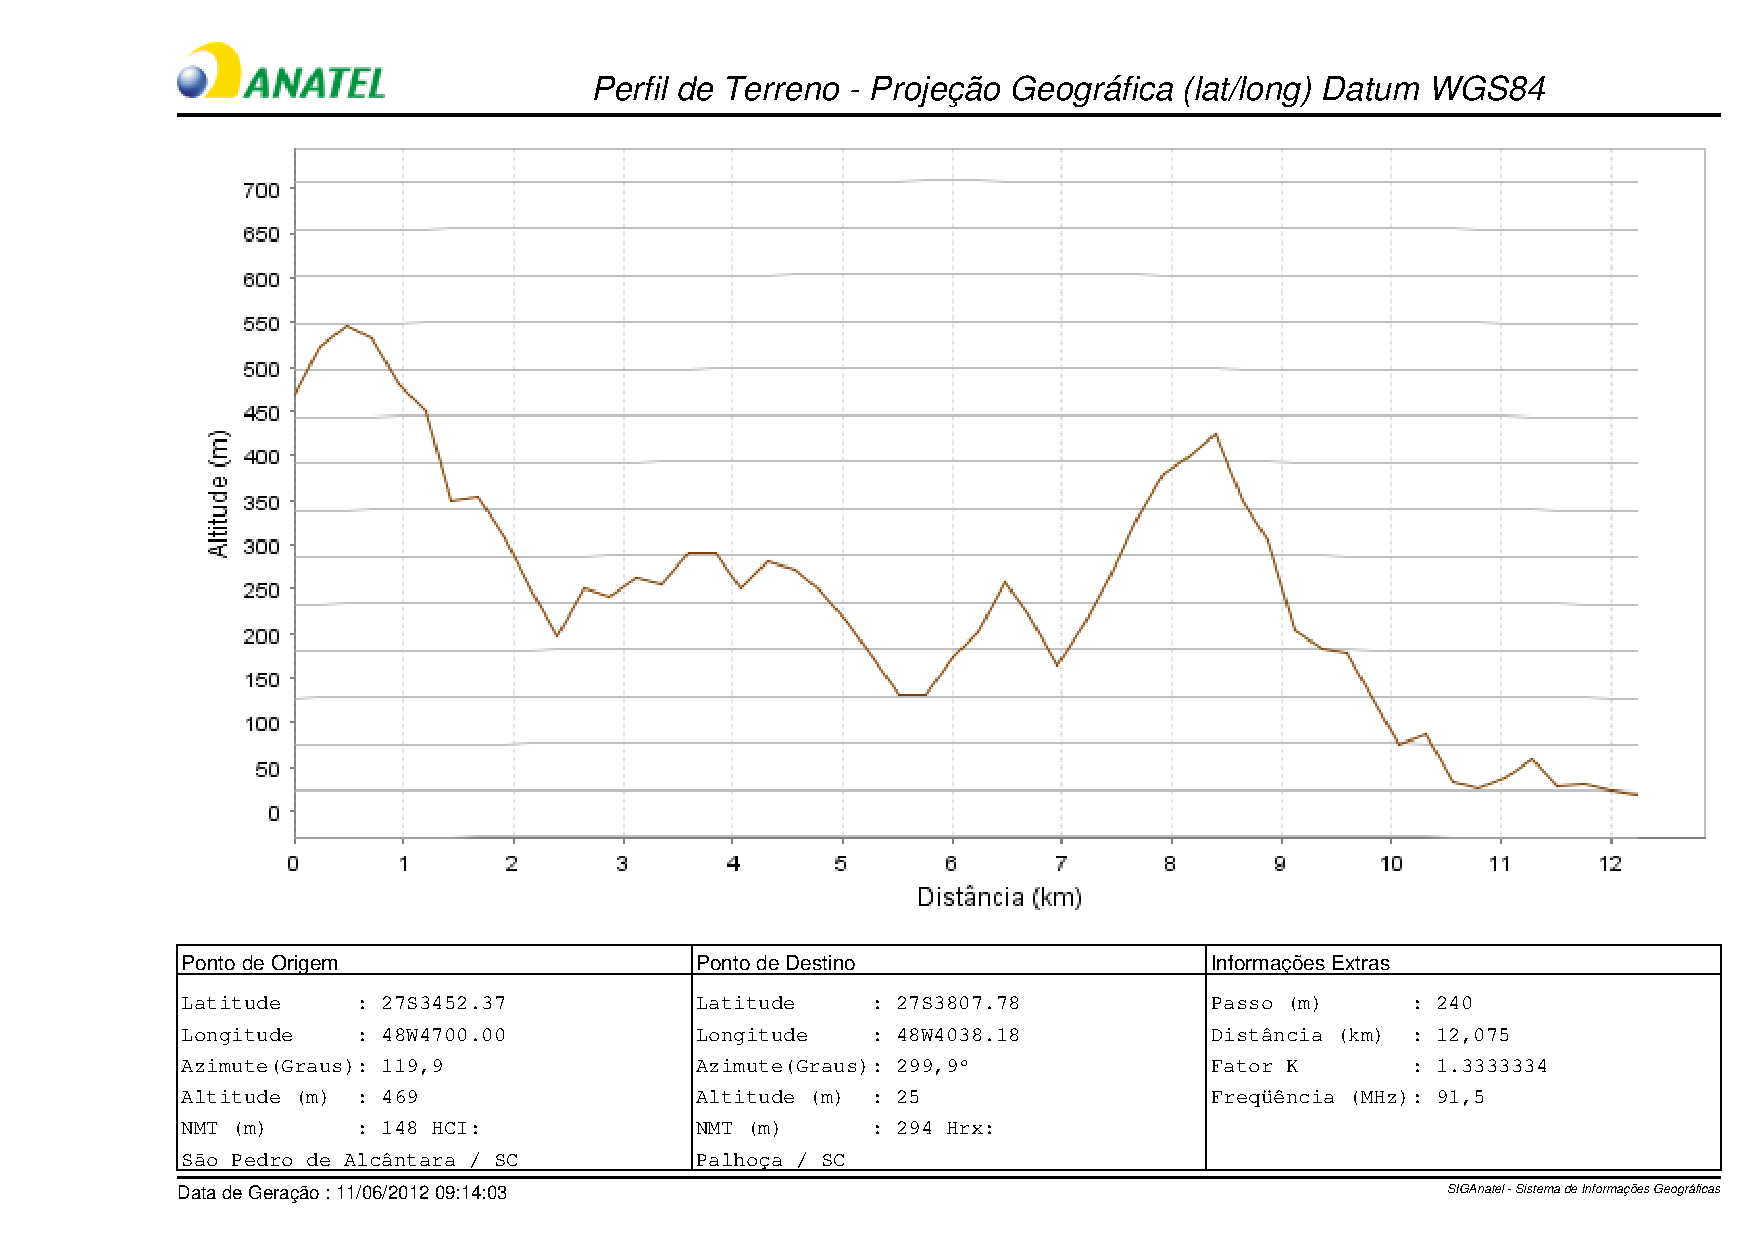
\includegraphics[scale=.5]{./figuras/nmt5_v2.pdf} %Opções width (largura em pt ou cm ou vezes se não houver unidade de medida), height (altura em pt, cm ou vezes se não houver unidade de medida), angle (rotação em graus), scale (escala em vezes 0.5= 50%,1.5=150%, etc )

%\caption{Radial 5}
Radial 5
\end{center}
\label{nmt5}
\end{figure}

\begin{figure}[ht] % [especificador de posições]:exemplos [htbp] - h:aqui, t:topo, b:baixo, p:página especial, !: desconsiderar parâmetros internos
\begin{center}
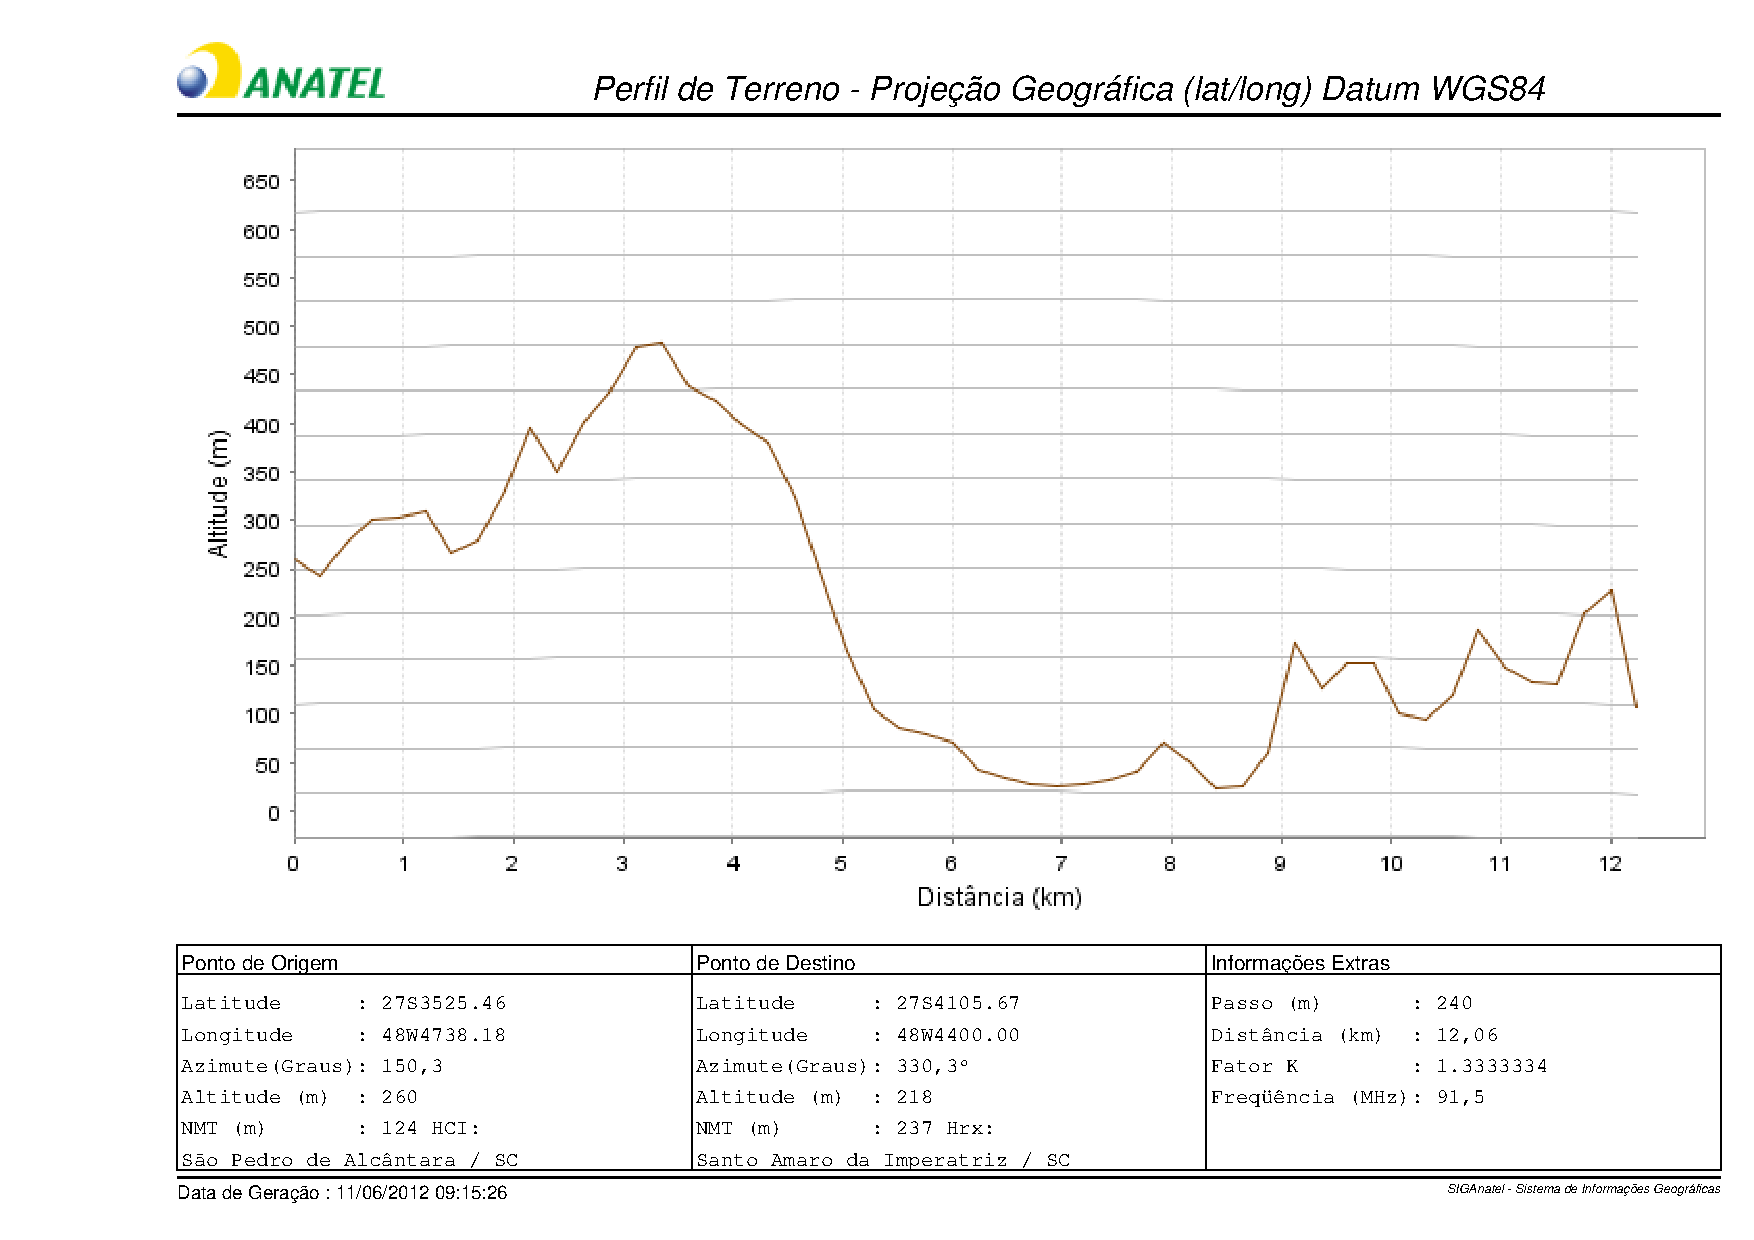
\includegraphics[scale=.5]{./figuras/nmt6_v2.pdf} %Opções width (largura em pt ou cm ou vezes se não houver unidade de medida), height (altura em pt, cm ou vezes se não houver unidade de medida), angle (rotação em graus), scale (escala em vezes 0.5= 50%,1.5=150%, etc )

%\caption{Radial 6}
Radial 6
\end{center}
\label{nmt6}
\end{figure}

\begin{figure}[ht] % [especificador de posições]:exemplos [htbp] - h:aqui, t:topo, b:baixo, p:página especial, !: desconsiderar parâmetros internos
\begin{center}
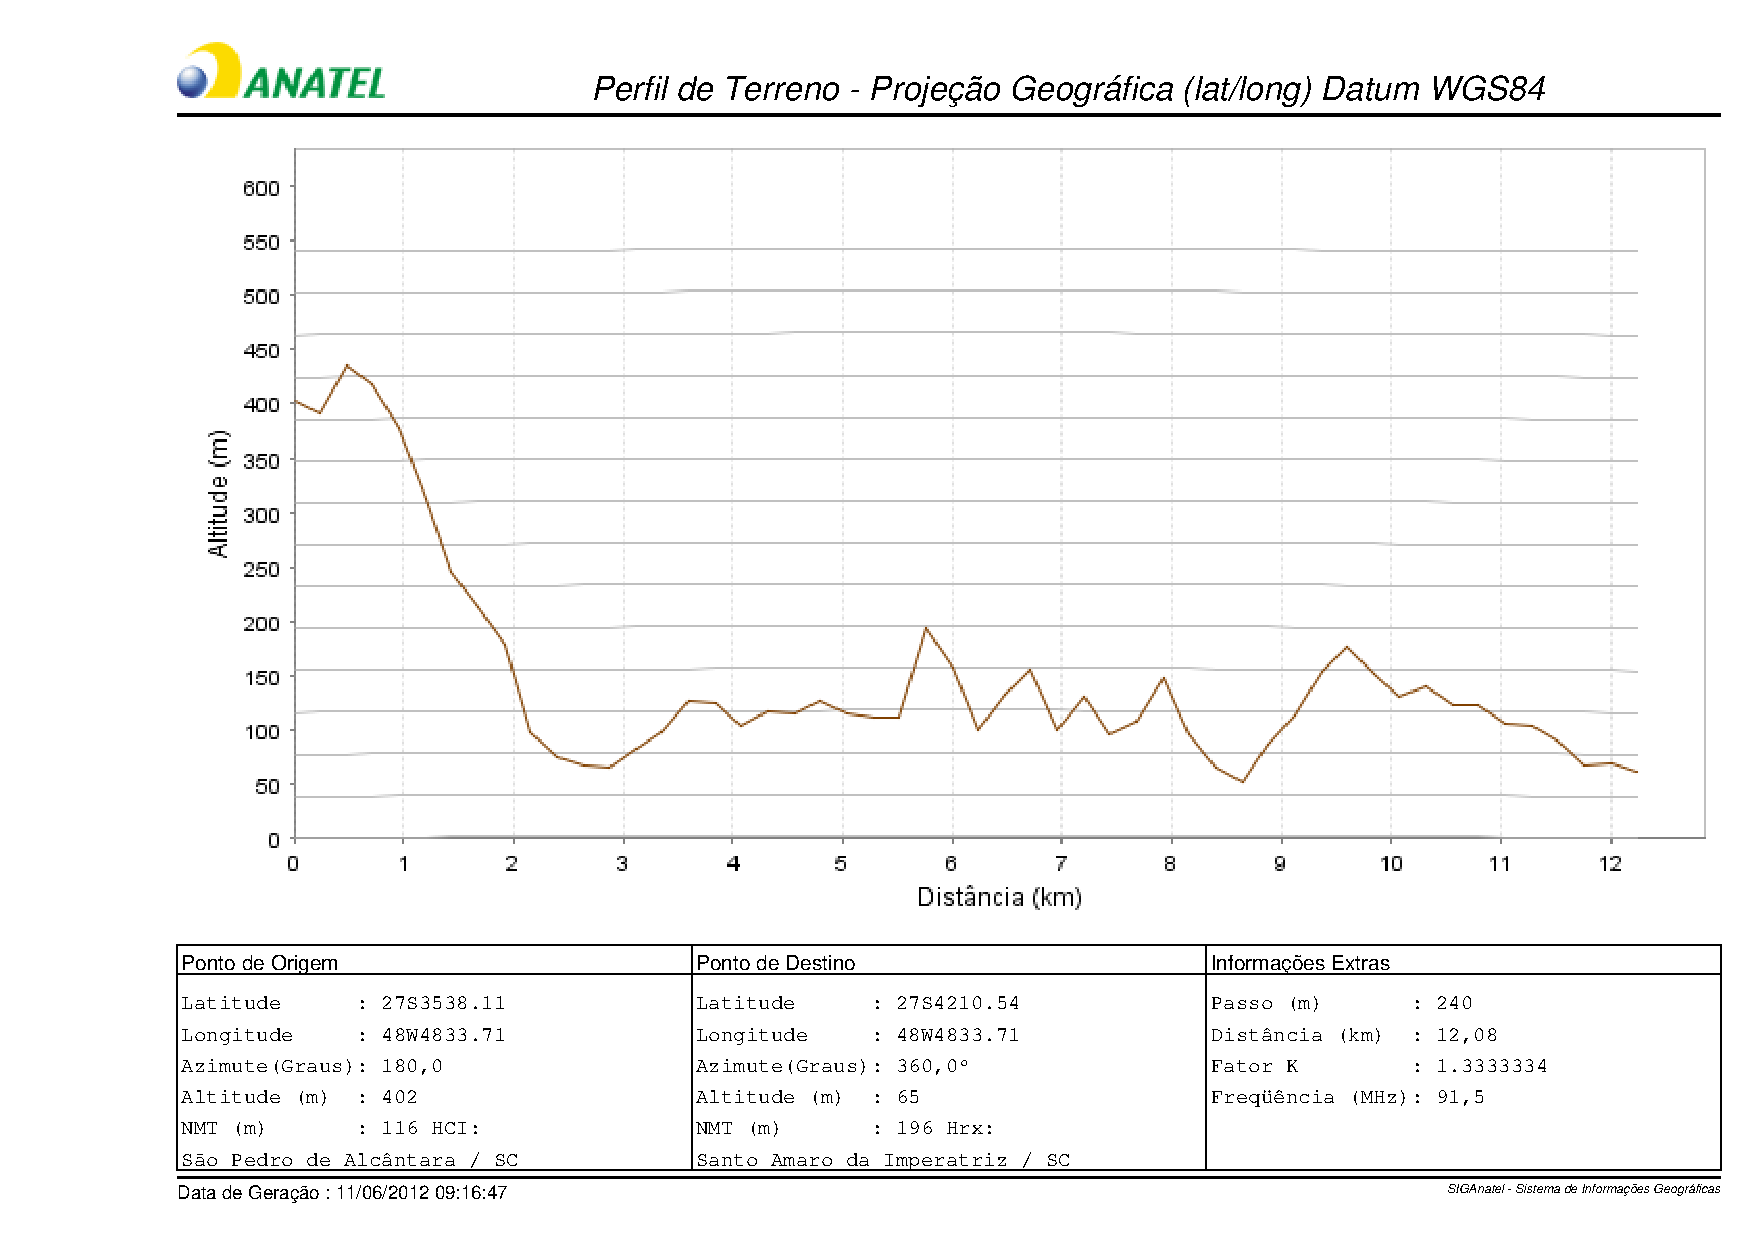
\includegraphics[scale=.5]{./figuras/nmt7_v2.pdf} %Opções width (largura em pt ou cm ou vezes se não houver unidade de medida), height (altura em pt, cm ou vezes se não houver unidade de medida), angle (rotação em graus), scale (escala em vezes 0.5= 50%,1.5=150%, etc )

%\caption{Radial 7}
Radial 7
\end{center}
\label{nmt7}
\end{figure}

\begin{figure}[ht] % [especificador de posições]:exemplos [htbp] - h:aqui, t:topo, b:baixo, p:página especial, !: desconsiderar parâmetros internos
\begin{center}
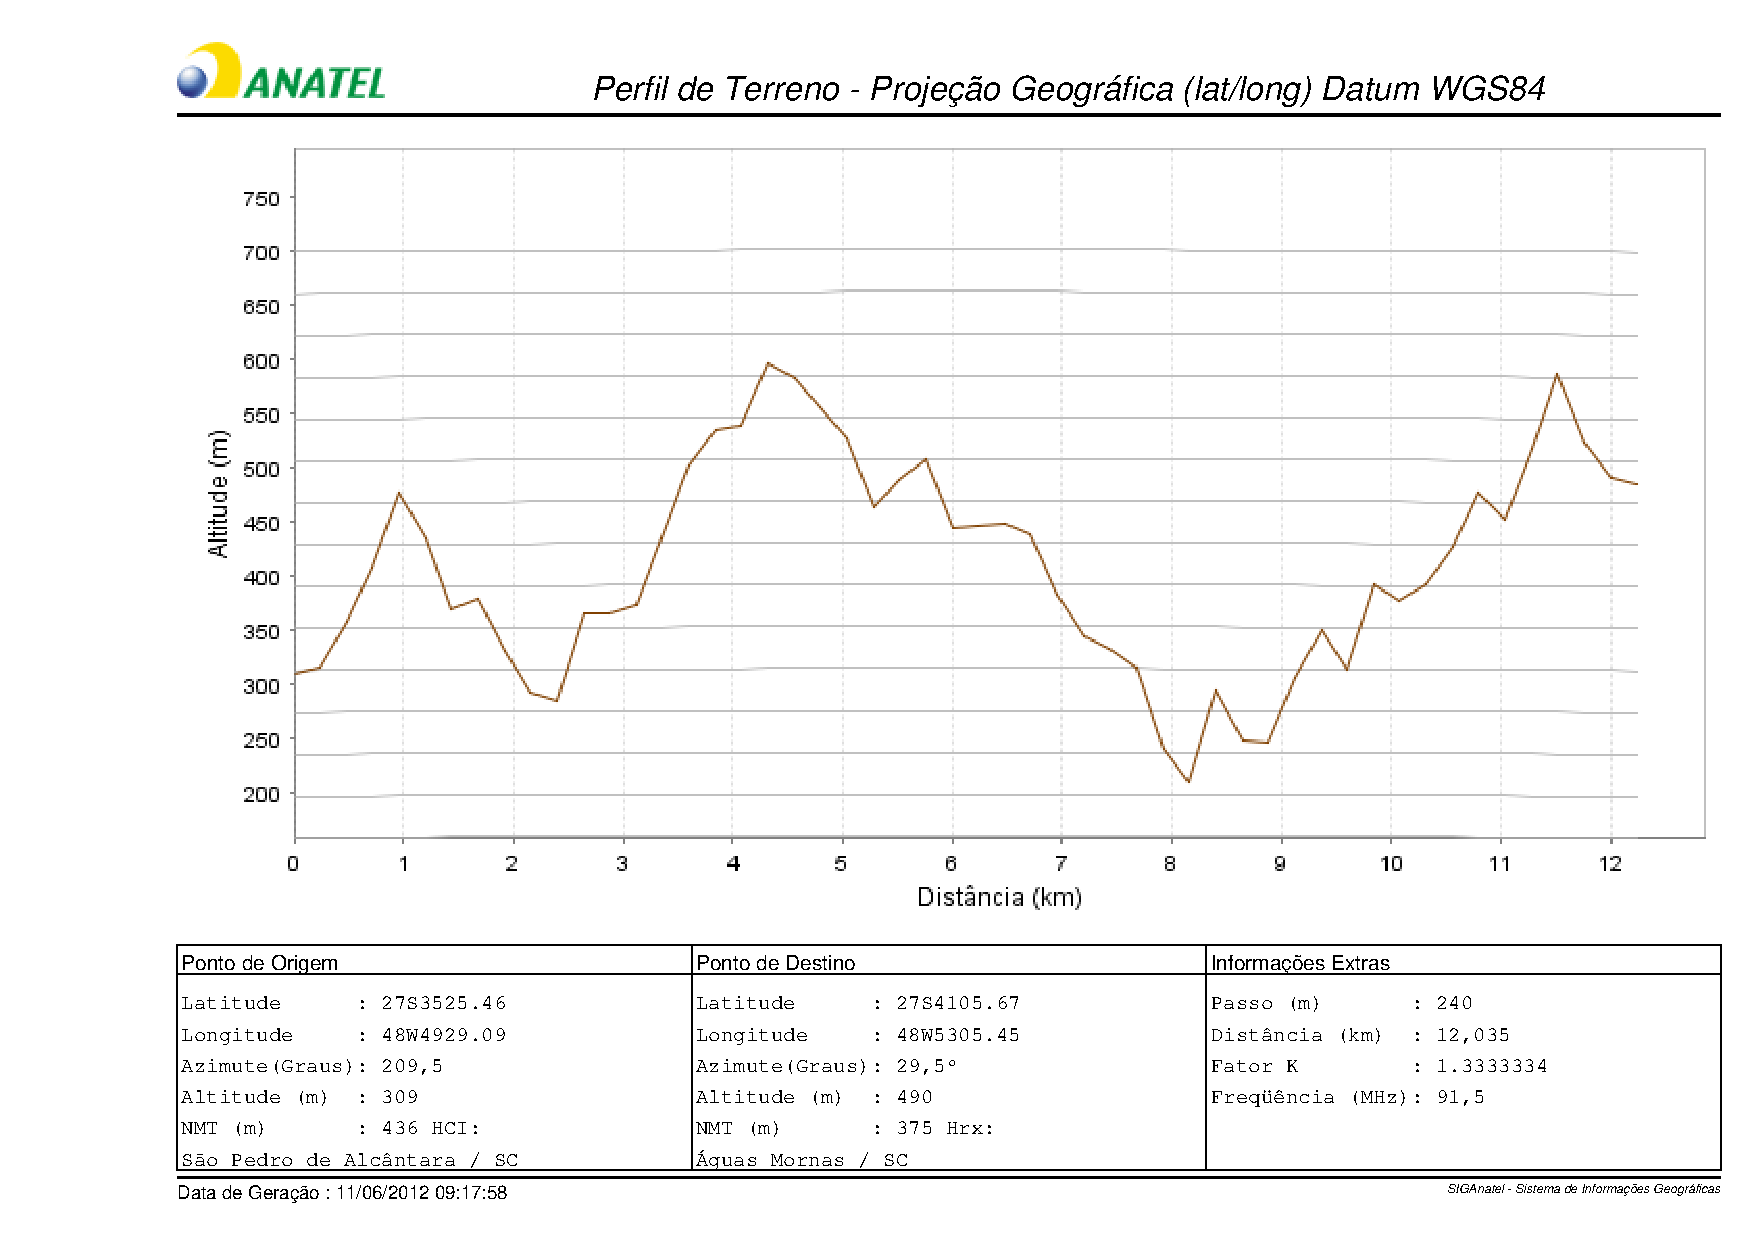
\includegraphics[scale=.5]{./figuras/nmt8_v2.pdf} %Opções width (largura em pt ou cm ou vezes se não houver unidade de medida), height (altura em pt, cm ou vezes se não houver unidade de medida), angle (rotação em graus), scale (escala em vezes 0.5= 50%,1.5=150%, etc )

%\caption{Radial 8}
Radial 8
\end{center}
\label{nmt8}
\end{figure}

\begin{figure}[ht] % [especificador de posições]:exemplos [htbp] - h:aqui, t:topo, b:baixo, p:página especial, !: desconsiderar parâmetros internos
\begin{center}
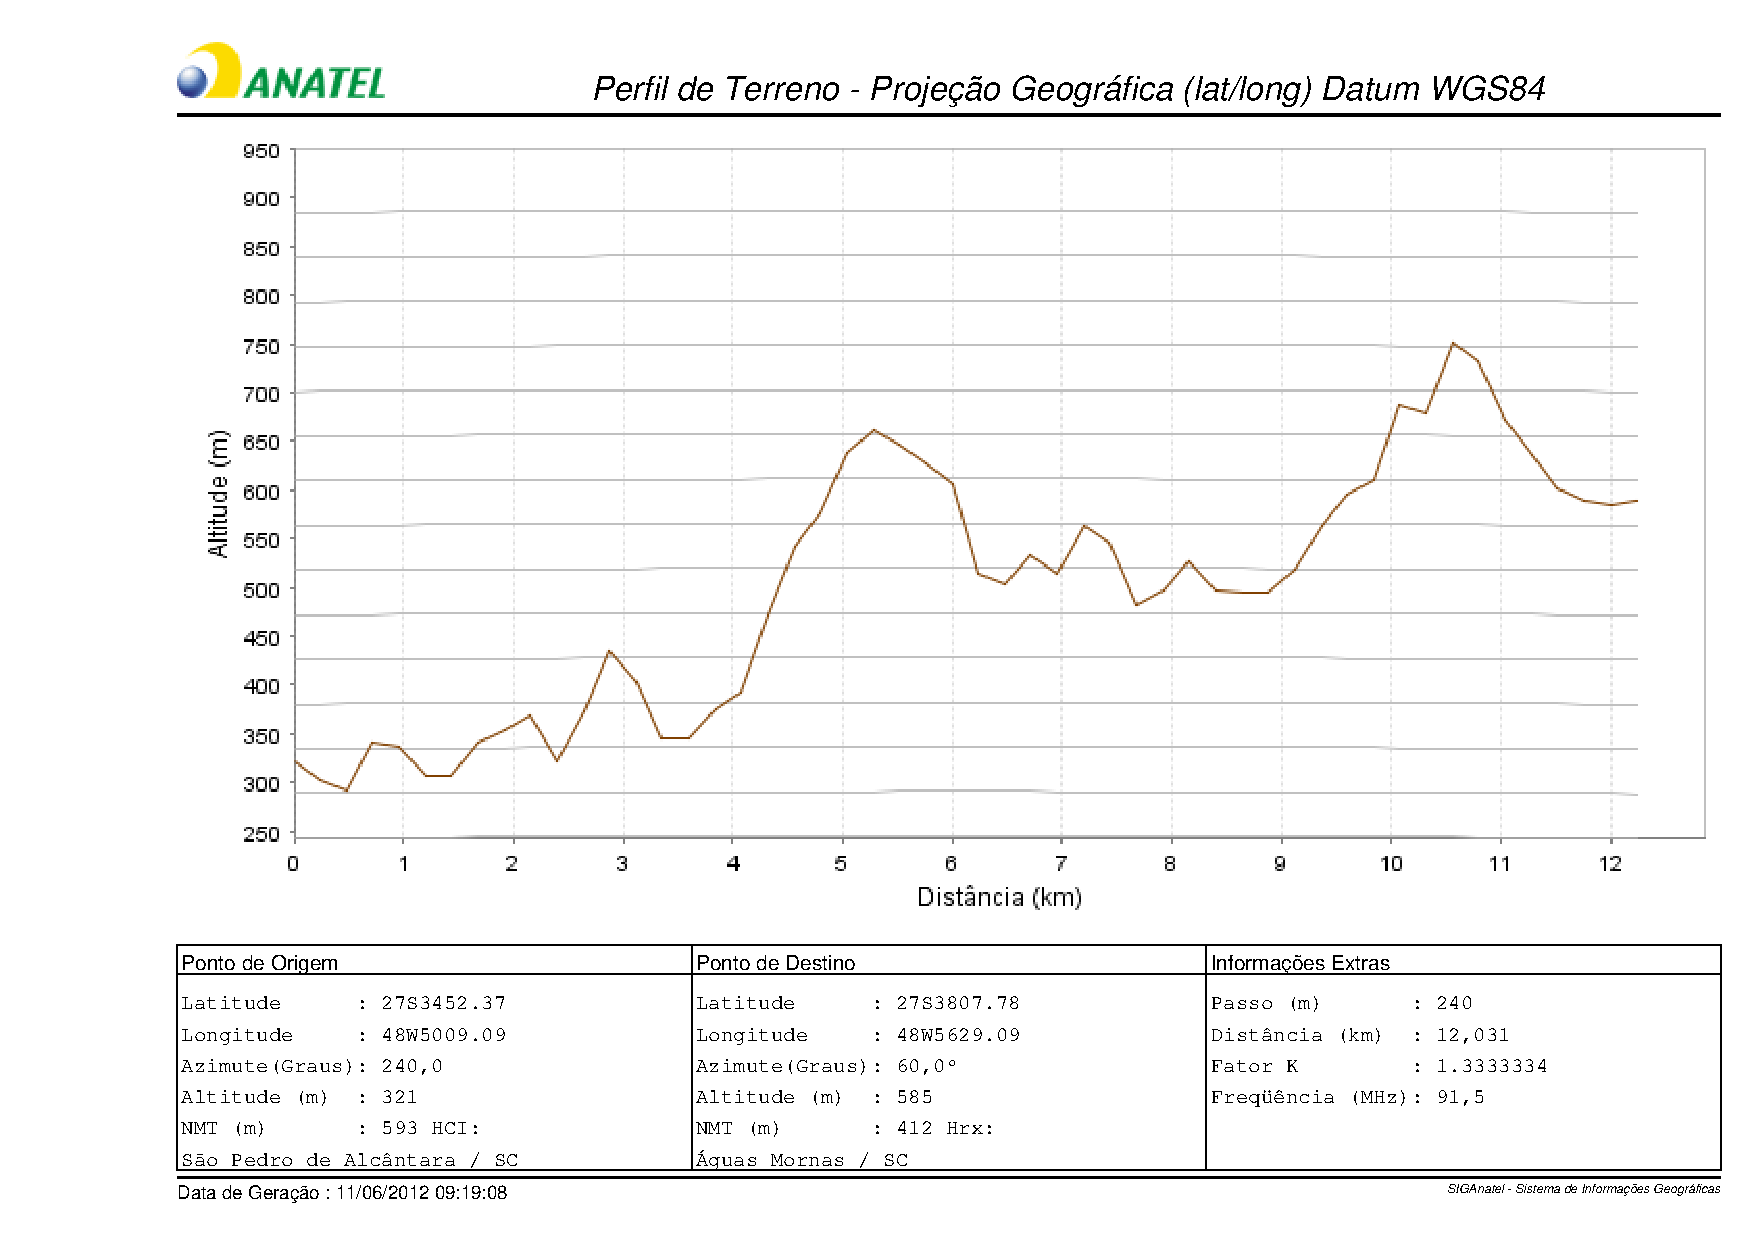
\includegraphics[scale=.5]{./figuras/nmt9_v2.pdf} %Opções width (largura em pt ou cm ou vezes se não houver unidade de medida), height (altura em pt, cm ou vezes se não houver unidade de medida), angle (rotação em graus), scale (escala em vezes 0.5= 50%,1.5=150%, etc )

%\caption{Radial 9}
Radial 9
\end{center}
\label{nmt9}
\end{figure}

\begin{figure}[ht] % [especificador de posições]:exemplos [htbp] - h:aqui, t:topo, b:baixo, p:página especial, !: desconsiderar parâmetros internos
\begin{center}
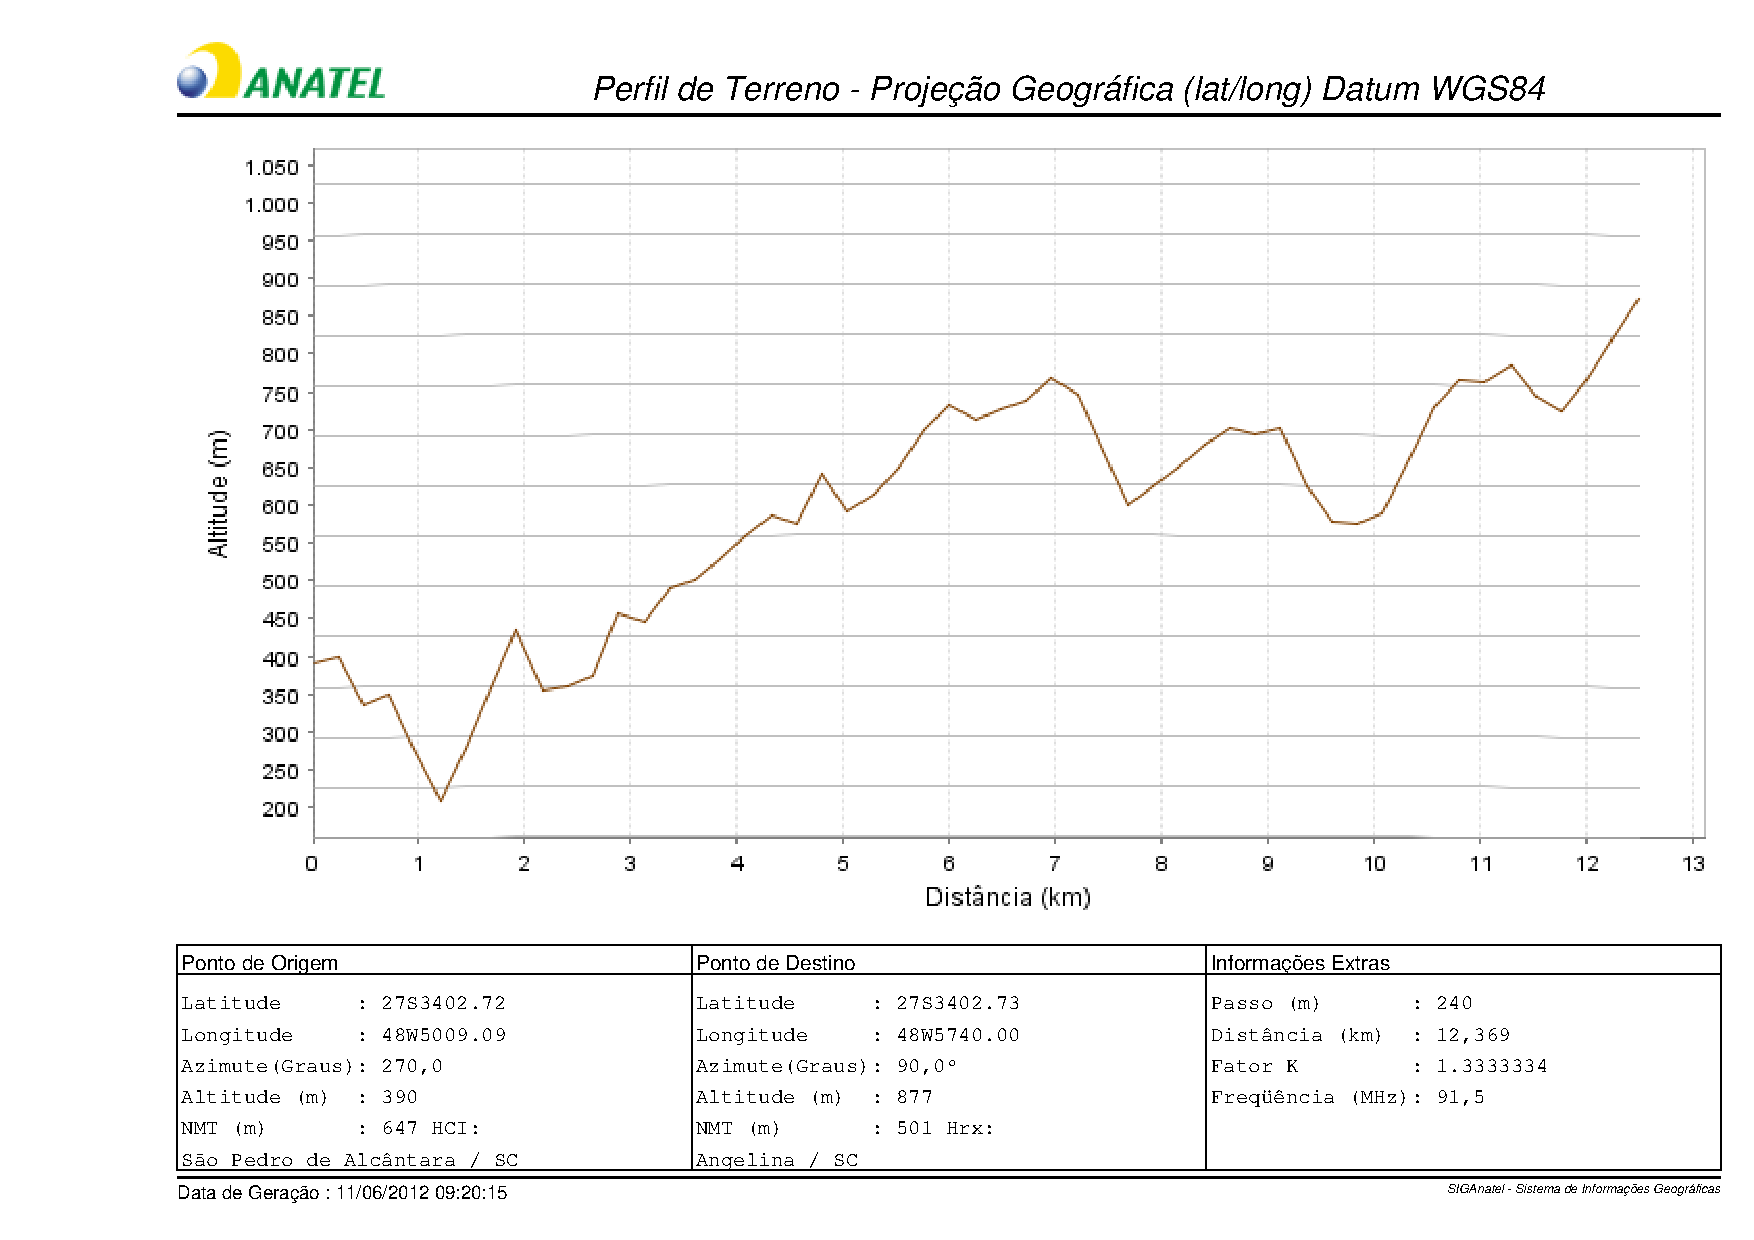
\includegraphics[scale=.5]{./figuras/nmt10_v2.pdf} %Opções width (largura em pt ou cm ou vezes se não houver unidade de medida), height (altura em pt, cm ou vezes se não houver unidade de medida), angle (rotação em graus), scale (escala em vezes 0.5= 50%,1.5=150%, etc )

%\caption{Radial 10}
Radial 10
\end{center}
\label{nmt10}
\end{figure}

\begin{figure}[ht] % [especificador de posições]:exemplos [htbp] - h:aqui, t:topo, b:baixo, p:página especial, !: desconsiderar parâmetros internos
\begin{center}
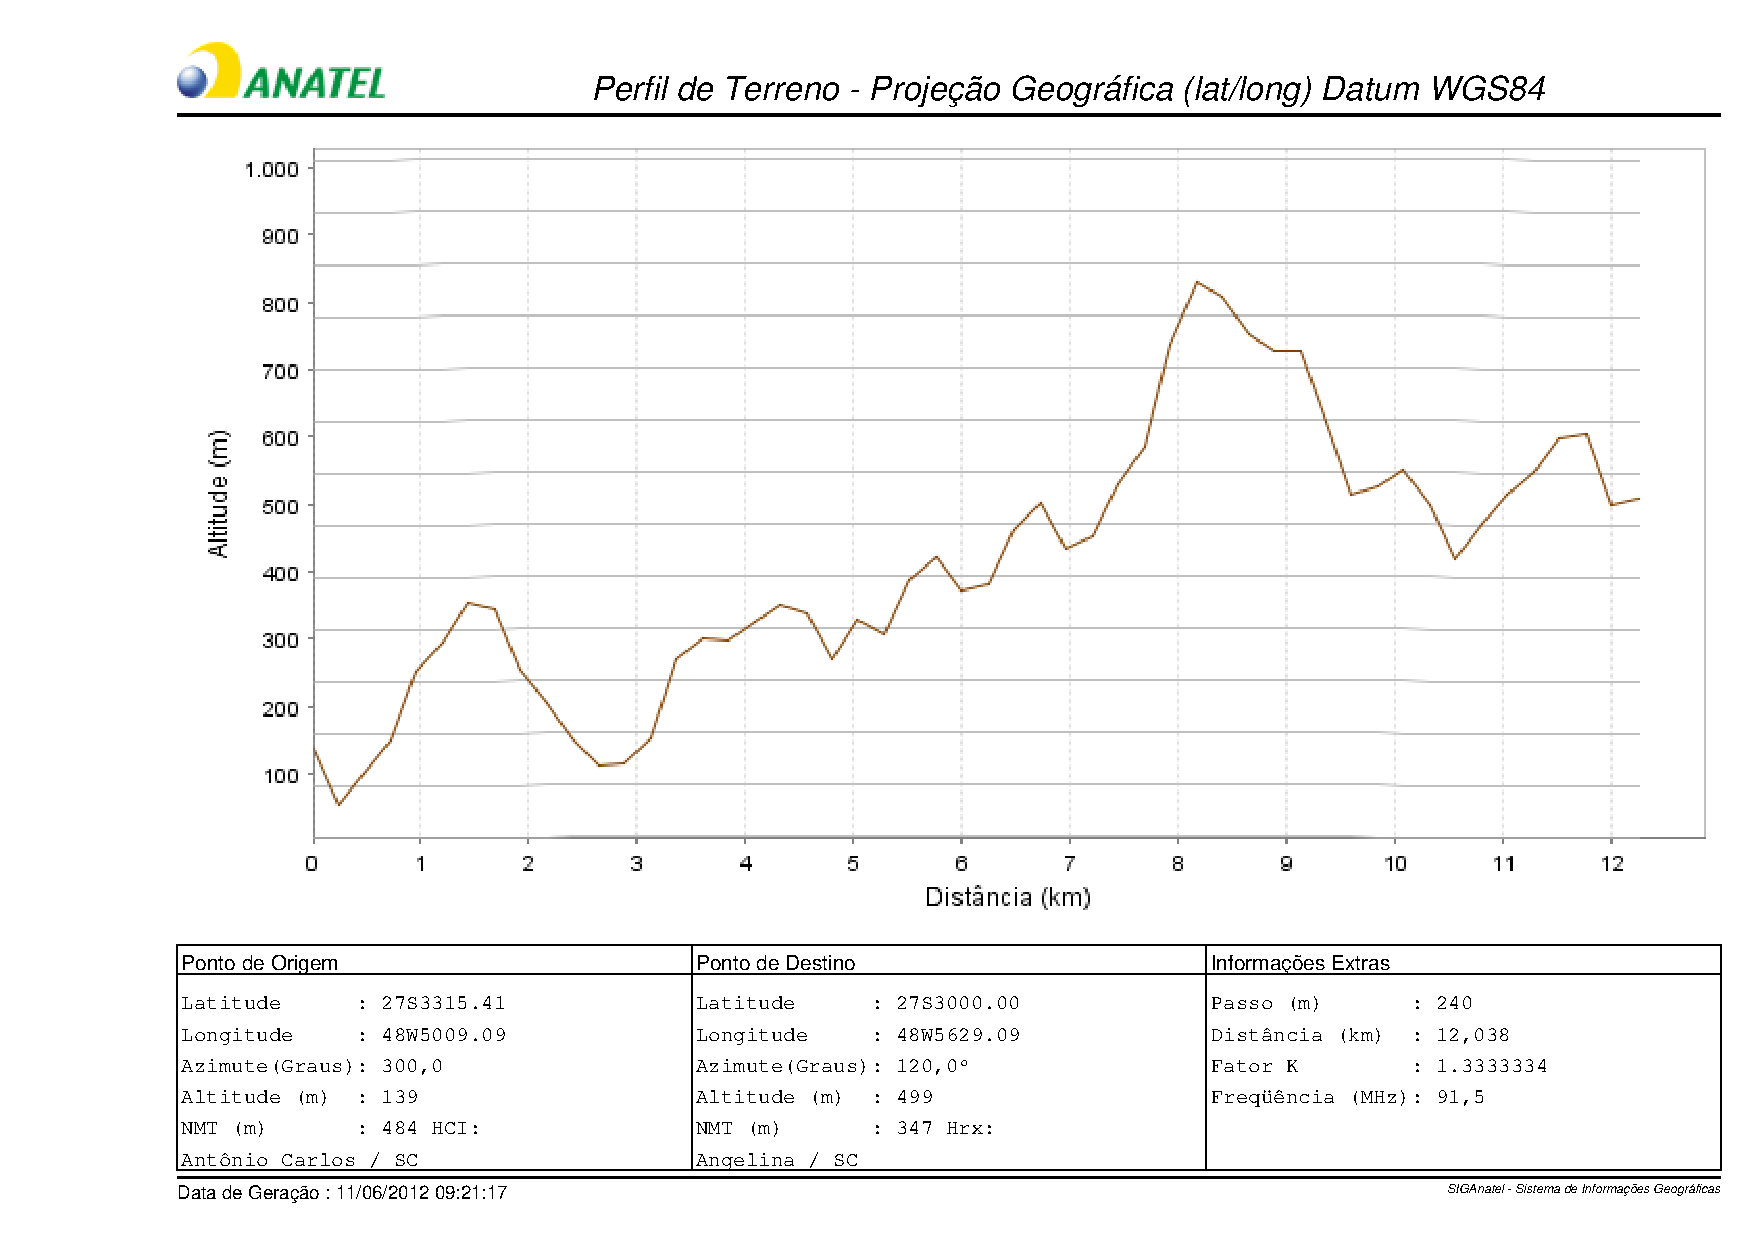
\includegraphics[scale=.5]{./figuras/nmt11_v2.pdf} %Opções width (largura em pt ou cm ou vezes se não houver unidade de medida), height (altura em pt, cm ou vezes se não houver unidade de medida), angle (rotação em graus), scale (escala em vezes 0.5= 50%,1.5=150%, etc )

%\caption{Radial 11}
Radial 11
\end{center}
\label{nmt11}
\end{figure}

\begin{figure}[ht] % [especificador de posições]:exemplos [htbp] - h:aqui, t:topo, b:baixo, p:página especial, !: desconsiderar parâmetros internos
\begin{center}
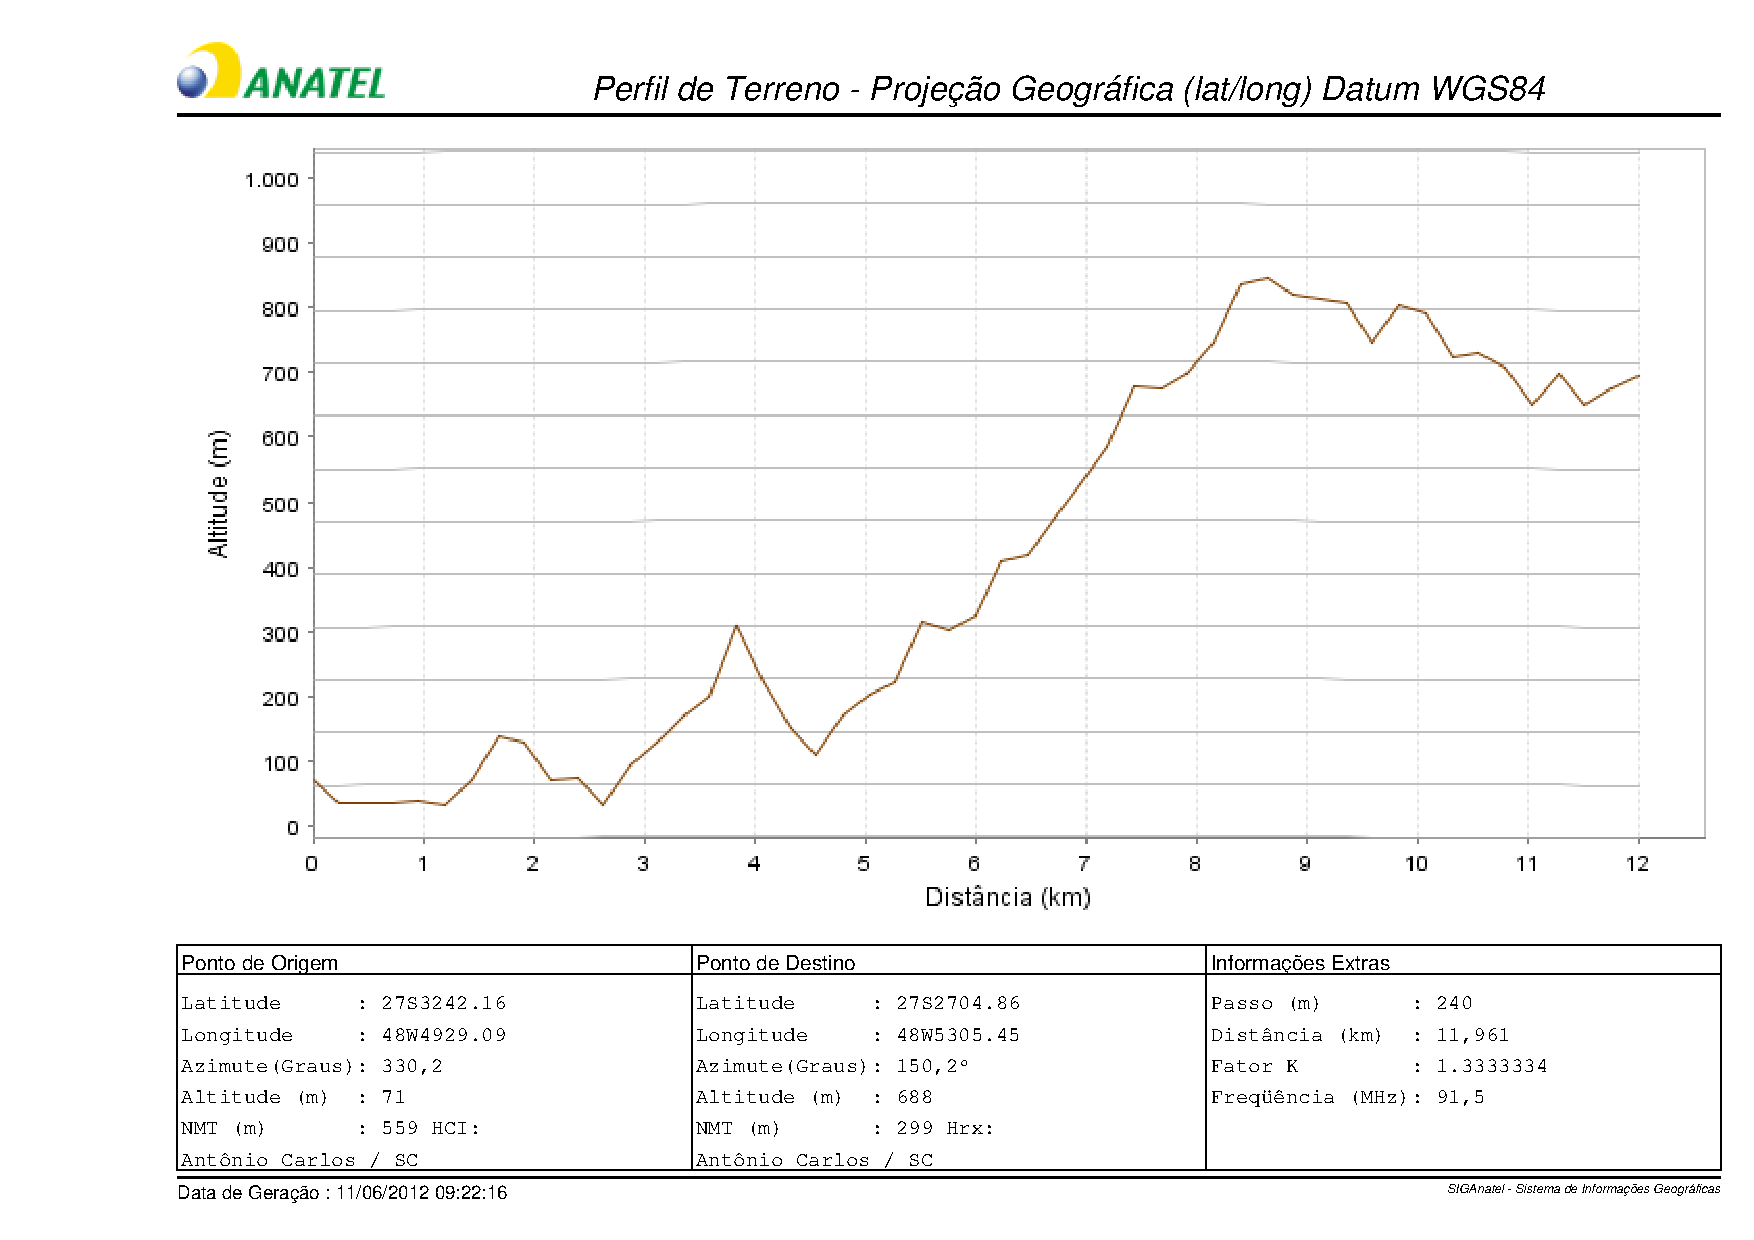
\includegraphics[scale=.5]{./figuras/nmt12_v2.pdf} %Opções width (largura em pt ou cm ou vezes se não houver unidade de medida), height (altura em pt, cm ou vezes se não houver unidade de medida), angle (rotação em graus), scale (escala em vezes 0.5= 50%,1.5=150%, etc )

%\caption{Radial 12}
Radial 12
\end{center}
\label{nmt12}
\end{figure}

